\providecommand{\main}{../../../..}
\documentclass[\main/dresen_thesis.tex]{subfiles}
\begin{document}
  \label{sec:looselyPackedNS:layers:pnr}
  With polarized neutron reflectometry it is possible to probe the magnetic structure of the spin-coated nanosphere layers with depth-resolution.
  For this purpose the samples SC-IOS-11 and SC-IOS-7 were extensively studied at SuperADAM at room temperature and $30 \unit{K}$.
  To evaluate the reflectivity of the respective polarization channel, the nuclear structure is fixed to the scattering length profile obtained for the sample in the superparamagnetic state at zero field.
  The magnetic splitting of the reflectivity curves is then described only by the magnetic scattering length density profile, which directly correlates to the spin density of the sample.

  \paragraphNewLine{Polarized Reflectivity at 300 K}
  \begin{figure}[tb]
    \centering
    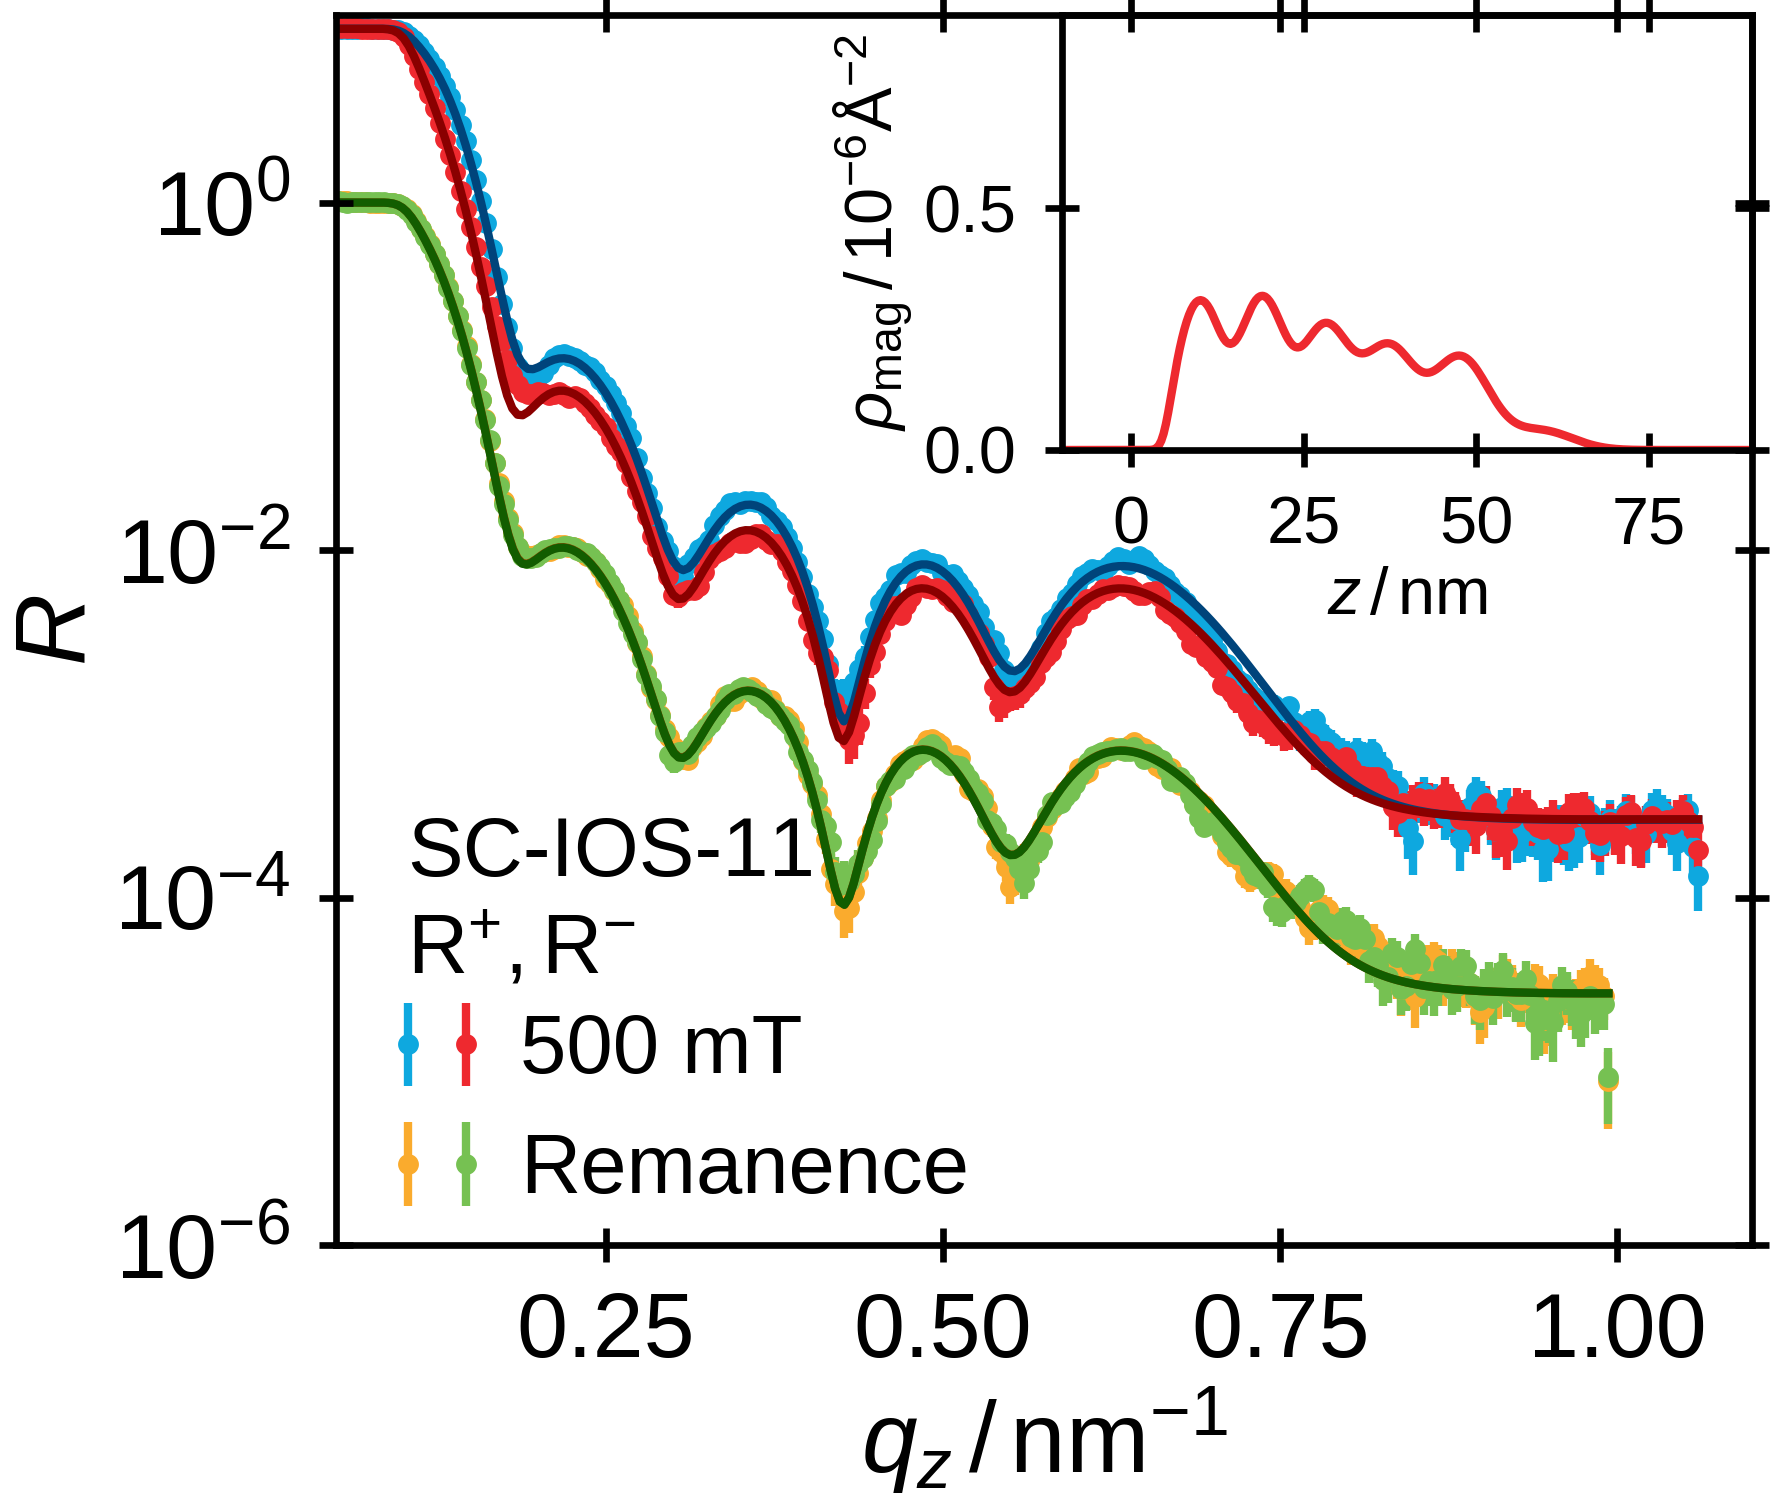
\includegraphics{looselyPackedNP_VerticalStructure_SC-IOS-11_PNR300K_500mT_HomogeneousModel}
    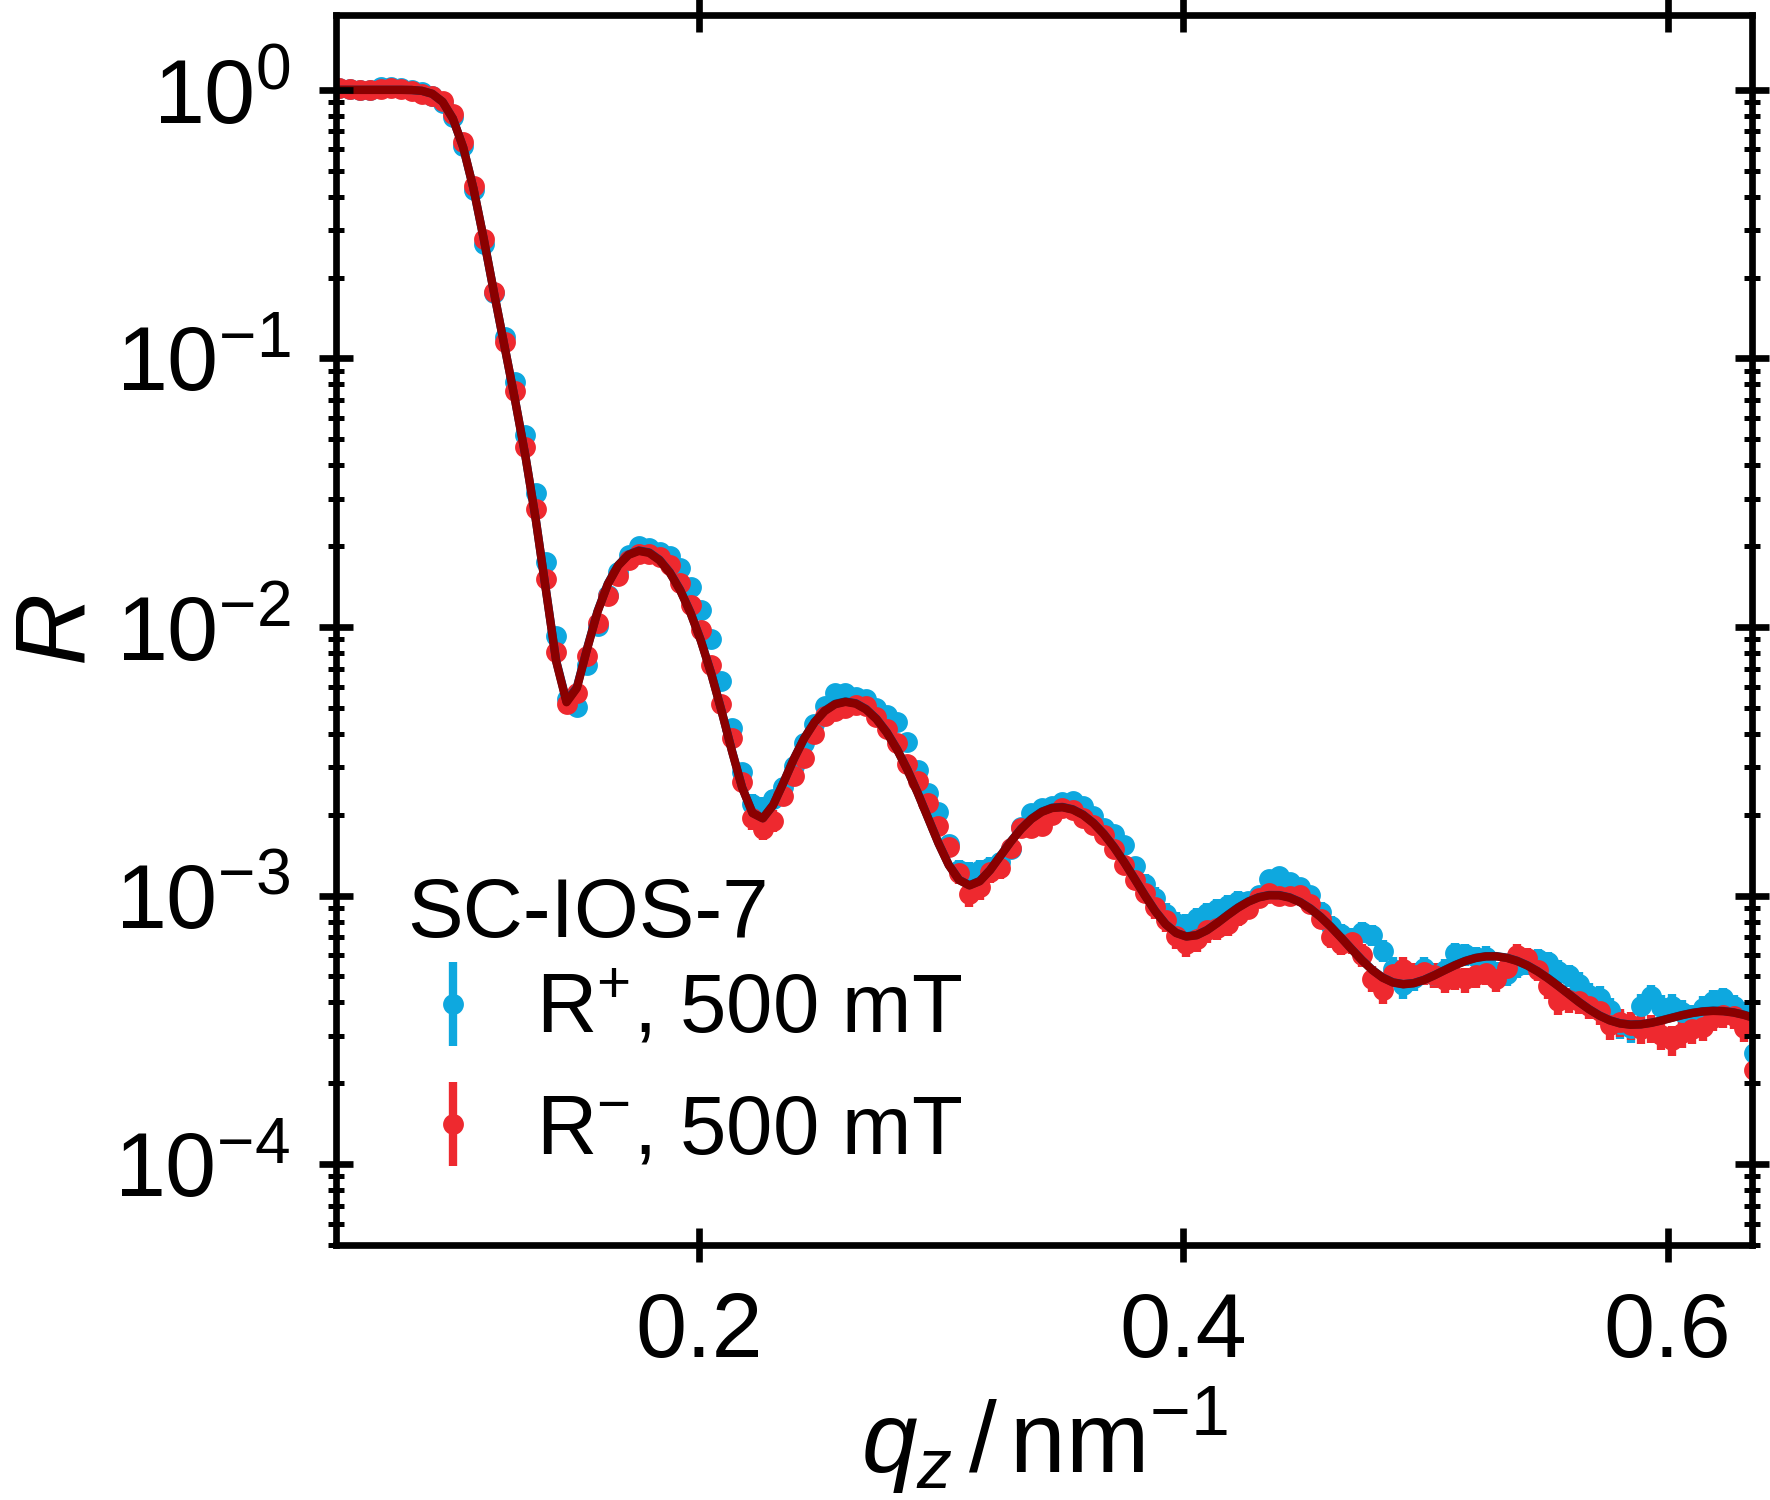
\includegraphics{looselyPackedNP_VerticalStructure_SC-IOS-7_PNR300K_500mT}
    \caption{\label{fig:looselyPackedNP:layer:pnrRoomTemperatureMagneticHomModel}Room temperature polarized neutron reflectivity ($R^{+},\, R^{-}$) of SC-IOS-11 (left) and SC-IOS-7 (right). For SC-IOS-11 the PNR measured after removal of the field at remanence is additionally shown. A scattering length density profile where each layer is homogeneously magnetized with the same magnetic scattering length density is fit.}
  \end{figure}
  In \reffig{fig:looselyPackedNP:layer:pnrRoomTemperatureMagneticHomModel} the reflectivity at room temperature and $500 \unit{mT}$ is shown for both SC-IOS-11 and SC-IOS-7, as well as the remanent state of SC-IOS-11 after removal of the magnetic field.
  For SC-IOS-7 no magnetic splitting of the two polarization channels is observed and thus the sample is still well described by only the nuclear scattering length density profile.
  On the other hand for SC-IOS-11 a significant contrast is visible between $R^{+}$ and $R^{-}$.
  In the inset of \reffig{fig:looselyPackedNP:layer:pnrRoomTemperatureMagneticHomModel}, it is assumed that the nanospheres in SC-IOS-11 are homogeneously magnetized and that no angle between the magnetization and neutron polarization $\gamma \eq 0 ^\circ$ is given.
  With these assumptions, the magnetic contrast can already be well described by only a single parameter for the magnetic scattering length density of the single spheres, $\rho_\mathrm{mag}^\mathrm{sphere} \eq 0.560(6) \cdot \unit{10^{-6} \angstrom^{-2}}$, which corresponds to a magnetization of $192(2) \unit{kA \, m^{-1}}$.
  This result is close to the value obtained for the sample by the complimentary VSM experiment at room temperature in \refsec{sec:looselyPackedNS:layer:vsm} of $206 \unit{kA \,m^{-1}}$, which raises confidence in the consistency of the scattering length density model of the sample.

  \begin{figure}[tb]
    \centering
    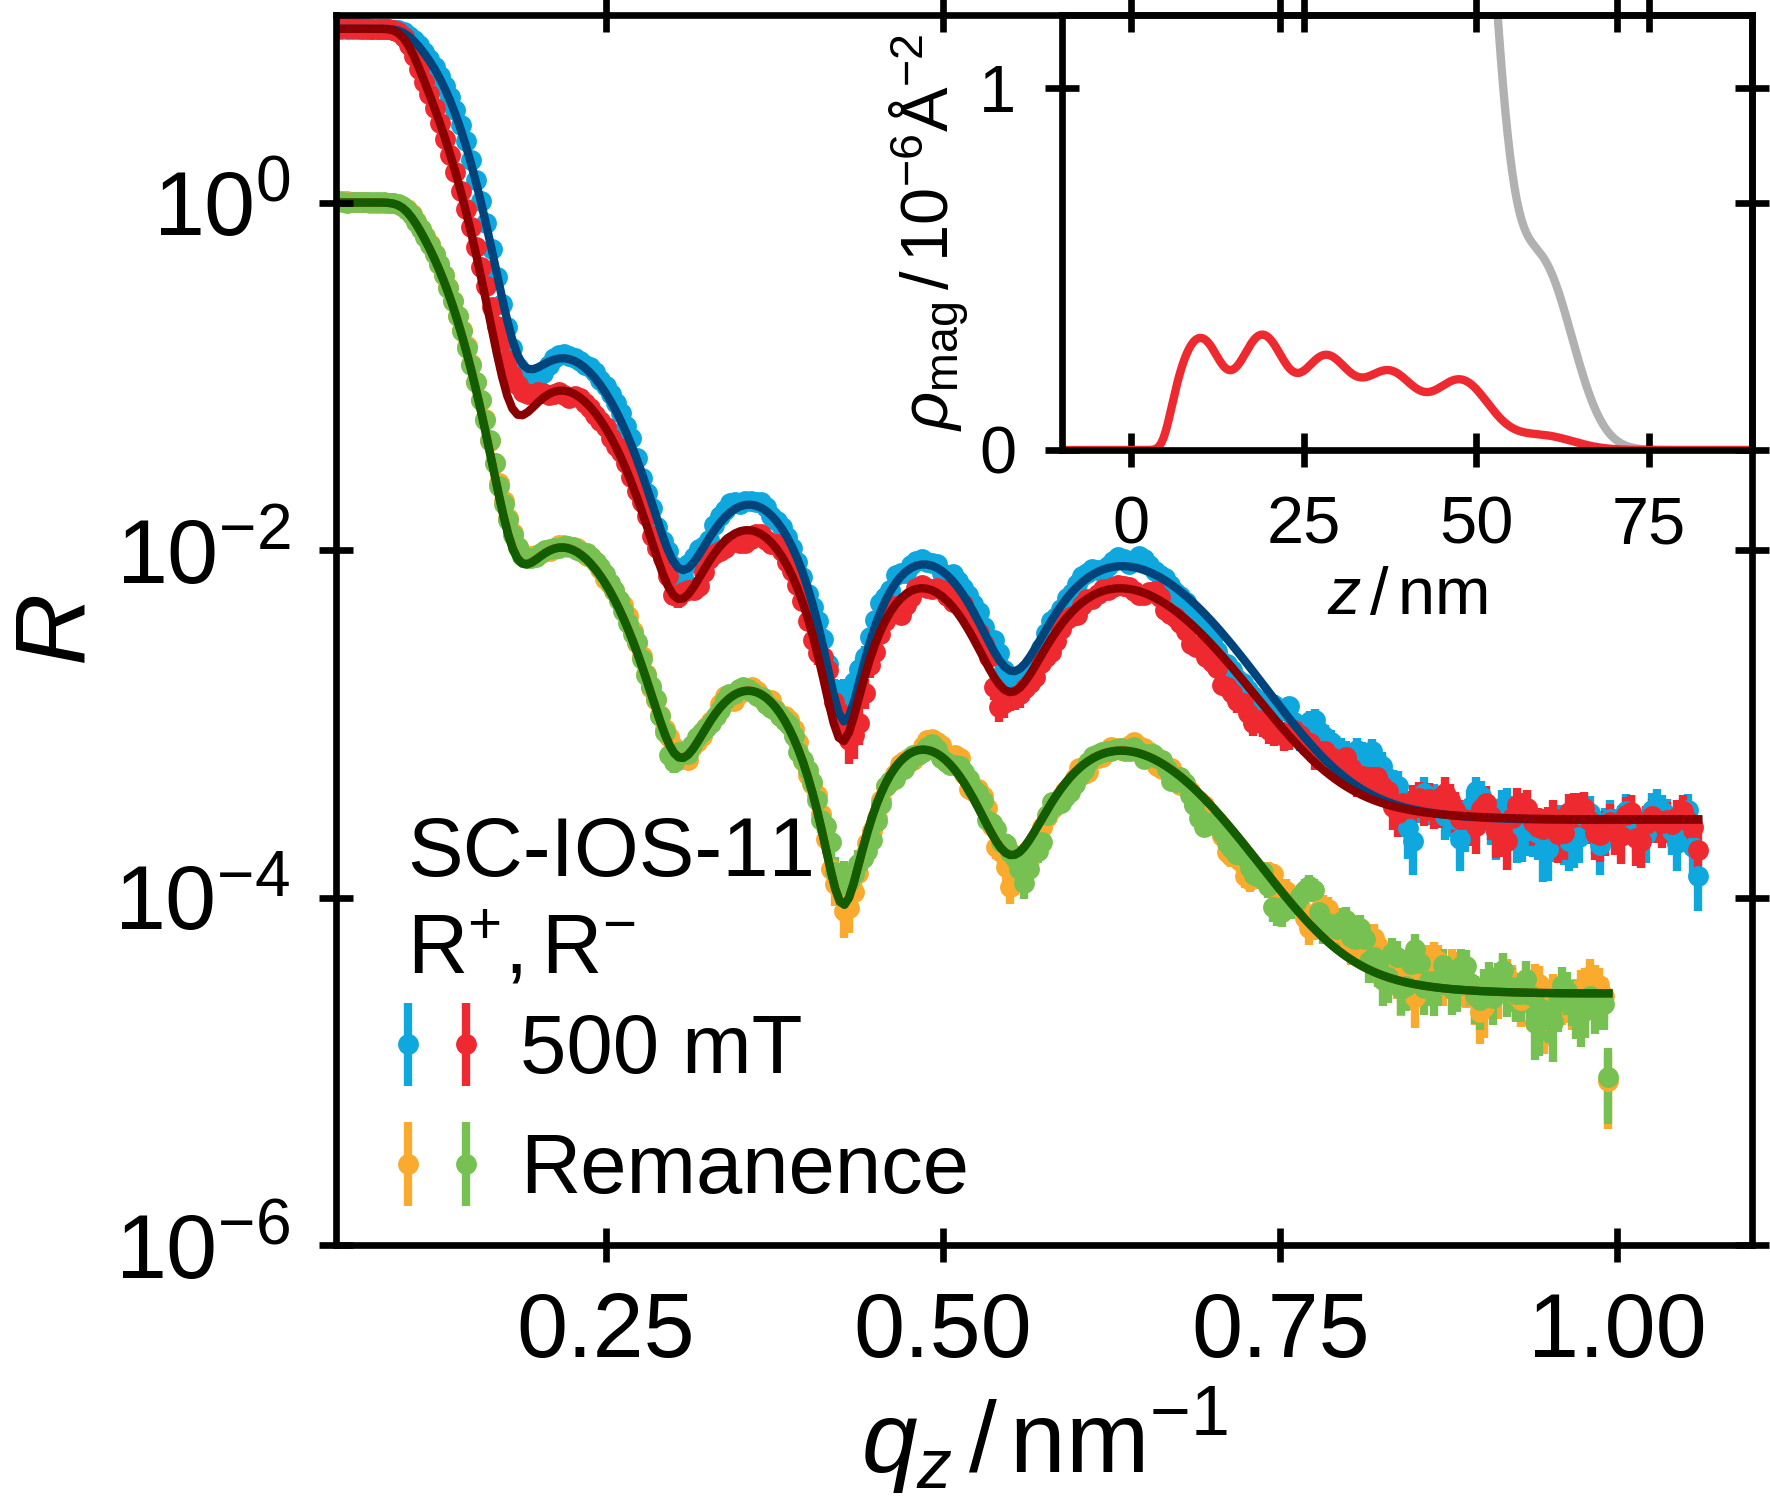
\includegraphics{looselyPackedNP_VerticalStructure_SC-IOS-11_PNR300K_500mT}
    \caption{\label{fig:looselyPackedNP:layer:pnrRoomTemperatureMagnetic}Room temperature PNR of SC-IOS-11, with the magnetic scattering length density of each layer fit independently.}
  \end{figure}
  As polarized neutron reflectometry allows to study the magnetization profile with depth-resolution, the respective layers have been further allowed to vary independently in magnetization density, shown in \reffig{fig:looselyPackedNP:layer:pnrRoomTemperatureMagnetic}.
  The obtained parameters are listed in comparison to the parameter of the homogeneously magnetized sample in \reftab{tab:looselyPackedNP:layers:pnrSCIOS300K500mT}.
  By the free variation, the fit of the calculated and experimental reflectivity can be further improved, which becomes visible in the reduced $\chi^2$.
  As a reduction of $\chi^2$ can also be achieved by simply adding more parameters to a model, another metric to evaluate the goodness-of-fit is the Bayesian information criterion (BIC), which penalizes the addition of parameters and where a decrease in $\Delta \mathrm{BIC} > 10$ is considered significant \cite{Schwarz_1978_Estim, Kass_1995_Bayes}.
  As a reduction of $\Delta \mathrm{BIC} \eq 347$ is observed, the model with the varied magnetization in the layers should be preferred.

  In the thereby obtained magnetic scattering length density profile, the lower layers have a reduced magnetization density, whereas the magnetization of the two higher layers is increased.
  A similar observation was made in literature by the study of Mishra \etal in \cite{Mishra_2012_Selfa} but not further discussed as in this study there is also no clear separation in the discussion between packing density and particle scattering length density.
  Comparing the magnetic scattering length profile, with the nuclear scattering length profile of SC-IOS-11, shown in \reffig{fig:looselyPackedNP:layer:reflectivity} (lower left), it can be seen that the packing density and the magnetic scattering length density of the nanospheres are inversely correlated.
  Meaning for the upper layers, which have a reduced packing density, the spin density is enhanced, whereas for the lower layers with closer packing, the spin density per layer is reduced.

  \begin{table}[!htbp]
    \centering
    \caption{\label{tab:looselyPackedNP:layers:pnrSCIOS300K500mT}Magnetization density of SC-IOS-11, assuming a homogeneously magnetized sample and for independently varied layer magnetizations. The index of $\rho_\mathrm{mag, i}$ counts from the lowest to the highest layer.}
    \begin{tabular}{ c | c | c | c | c}
      \rule{0pt}{2ex} \textbf{PNR \@ 300 K}  & \multicolumn{2}{c}{Hom. Magnetized} & \multicolumn{2}{c}{Varied Densities} \\
      \hline
      Layer     & $\rho_\mathrm{mag, i} \, / \unit{10^{-6} \angstrom^{-2}}$ & $M \, / \unit{kA \, m^{-1}}$ & $\rho_\mathrm{mag, i} \, / \unit{10^{-6} \angstrom^{-2}}$ & $M \, / \unit{kA \, m^{-1}}$\\
      \hline
      1         & \multirow{6}{*}{$0.560(6)$} & \multirow{6}{*}{$192(2)$}   & $0.49(2)$ & $168(7)$\\
      2         &                             &                             & $0.47(1)$ & $161(3)$\\
      3         &                             &                             & $0.56(2)$ & $192(7)$\\
      4         &                             &                             & $0.80(2)$ & $275(7)$\\
      5         &                             &                             & $1.13(4)$ & $388(14)$\\
      6         &                             &                             & $0.95(21)$& $326(72)$\\
      \hline
      $\chi^2$  & \multicolumn{2}{c}{$4.1$}   & \multicolumn{2}{c}{$2.0$}\\
      BIC       & \multicolumn{2}{c}{$768$}   & \multicolumn{2}{c}{$421$}\\
      \hline
    \end{tabular}
  \end{table}

  \paragraphNewLine{Polarized Reflectivity at 30 K}
  \begin{figure}[tb]
    \centering
    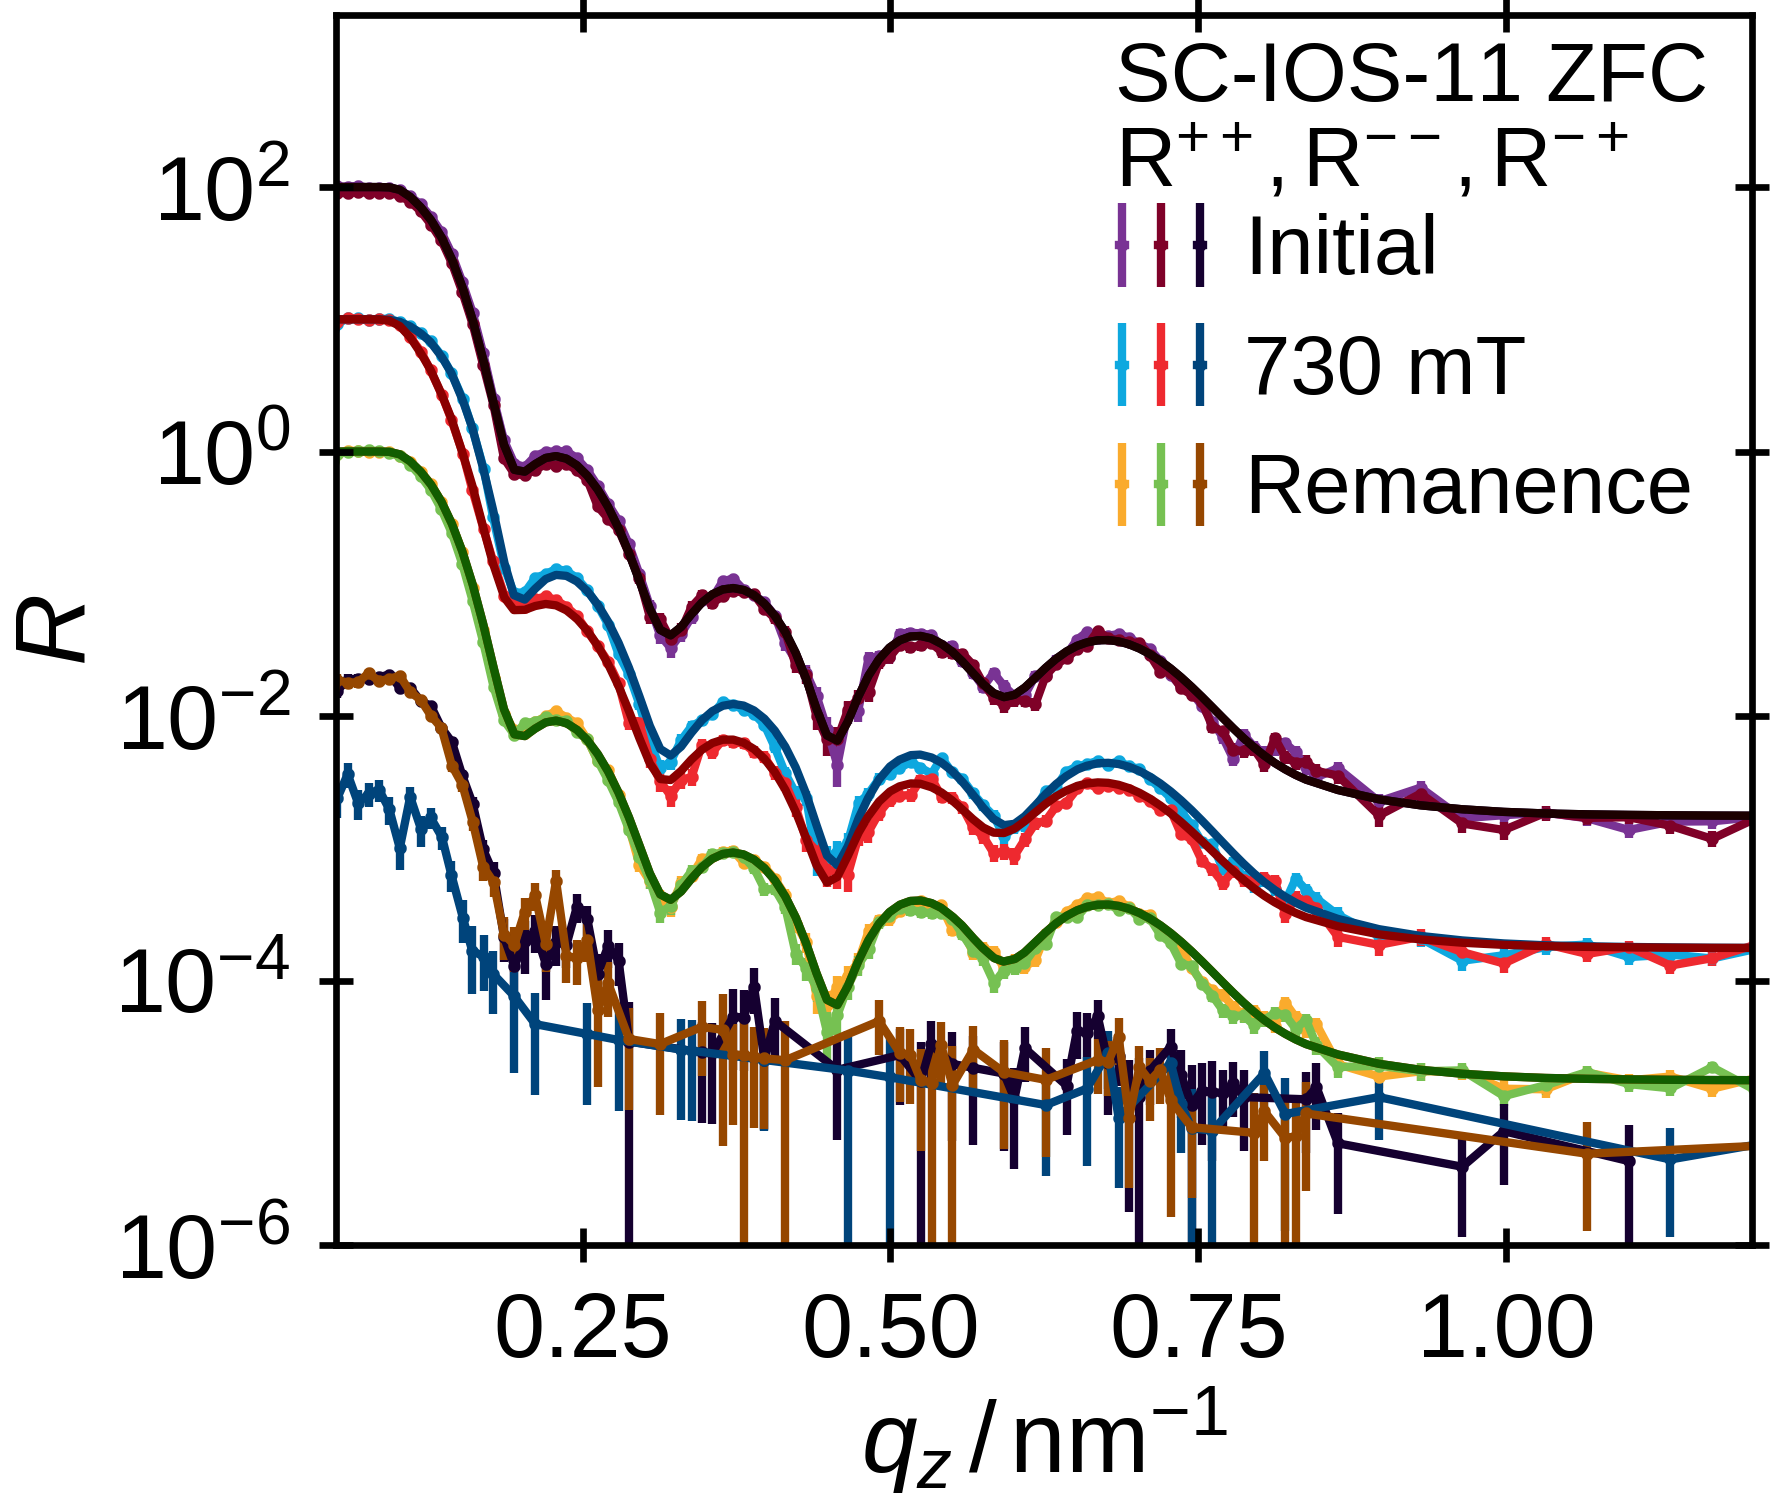
\includegraphics{looselyPackedNP_VerticalStructure_SC-IOS-11_PNR_ZFC30K}
    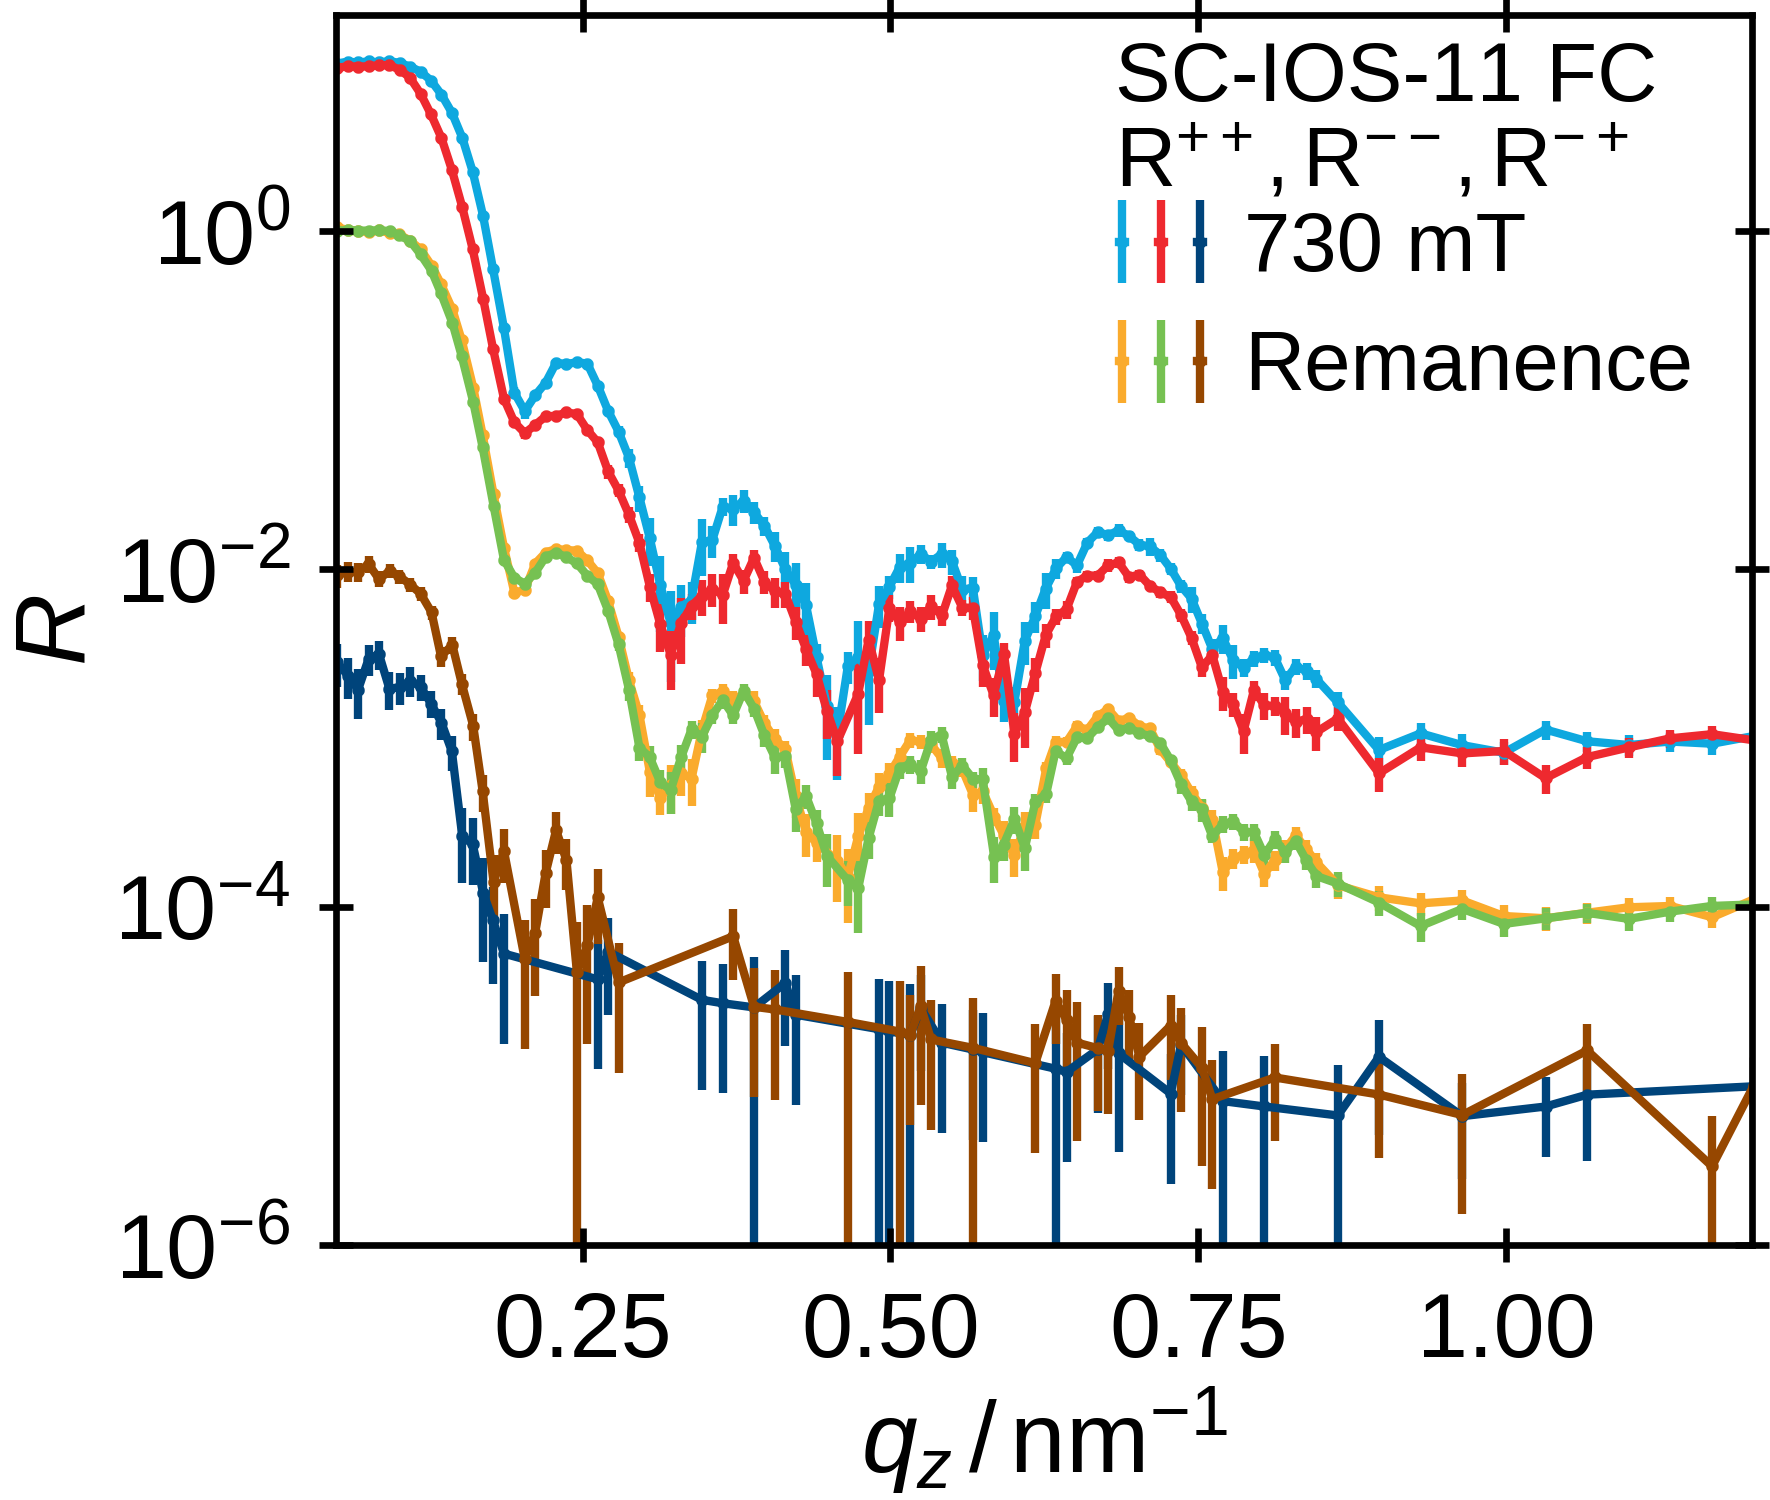
\includegraphics{looselyPackedNP_VerticalStructure_SC-IOS-11_PNR_FC30K}
    \caption{\label{fig:looselyPackedNP:layer:pnrZFCFCIOS11}Zero-field-cooled (left) and Field-cooled non-spin-flip reflectivity ($R^{++},\,R^{--}$) and spin-flip reflectivity ($R^{-+}$) of SC-IOS-11 at a magnetic field of $730 \unit{mT}$ and in remanence. For the zero-field cooled the initial reflectivity after cooling at guide field is additionally shown. The calculated curves for the initial state and the remanence states are from the purely nuclear model discussed in \refsec{sec:looselyPackedNS:layers:xrr}, and the magnetized reflectivities are calculated from independently varied layer magnetizations.}
  \end{figure}

  In \reffig{fig:looselyPackedNP:layer:pnrZFCFCIOS11} the reflectivities of SC-IOS-11 at $30 \unit{K}$ measured after zero-field cooling and field cooling are shown.
  The signal measured in the spin-flip channel is in all cases $<1-2 \%$ of the intensity measured in the non-spin-flip channels and can therefore only be attributed to spin-leakage due to the finite polarization efficiency of the instrument.
  This is intriguing for the case of the remanent magnetization.
  If the nanoparticular spins are super ferromagnetically coupled with one another and the zero magnetization at remanence were attributed to domain formation of the coupled spins, it would be expected that a significant signal is measured in the spin-flip channel due to spins aligning perpendicular to the neutron polarization in the sample plane, which is however not visible in the performed experiments.
  In an analogue experiment on magnetite nanospheres by Mishra \etal \cite{Mishra_2015_Polar}, the same result was observed at room temperature measurements and the authors concluded that the domains ordered on macroscopic stripes that are parallel to the original magnetization.

  To model the magnetization data, the nuclear scattering length density is used as determined from the initial ZFC data, and the magnetic scattering length density of the respective layers is fit in the same manner as was done for the room temperature measurement at $500 \unit{mT}$ in the previous paragraph.
  The remanence data, however, shows in all cases no magnetic splitting of the reflectivities and can therefore be well described by a purely nuclear scattering length density.
  The obtained values are tabulated in \reftab{tab:looselyPackedNP:layers:pnrSCIOS30K730mT}.

  \begin{table}[!htbp]
    \centering
    \caption{\label{tab:looselyPackedNP:layers:pnrSCIOS30K730mT}Low-temperature magnetization density of SC-IOS-11 for a homogeneously magnetized sample and for independently varied layer magnetizations. The index of $\rho_\mathrm{mag, i}$ counts from the lowest to the highest layer.}
    \begin{tabular}{ c | l | l}
      \rule{0pt}{2ex} \textbf{PNR \@ 30 K, 730 mT}  & ZFC & FC \\
      \hline
      $\rho_\mathrm{mag, 1} \, / \unit{10^{-6} \angstrom^{-2}} $ & $0.59(4)$ & $0.55(8)$\\
      $\rho_\mathrm{mag, 2} \, / \unit{10^{-6} \angstrom^{-2}} $ & $0.54(4)$ & $0.51(6)$\\
      $\rho_\mathrm{mag, 3} \, / \unit{10^{-6} \angstrom^{-2}} $ & $0.71(4)$ & $0.76(8)$\\
      $\rho_\mathrm{mag, 4} \, / \unit{10^{-6} \angstrom^{-2}} $ & $0.93(8)$ & $1.2(1)$\\
      $\rho_\mathrm{mag, 5} \, / \unit{10^{-6} \angstrom^{-2}} $ & $1.2(1)$  & $1.4(2)$\\
      $\rho_\mathrm{mag, 6} \, / \unit{10^{-6} \angstrom^{-2}} $ & $1.1(8)$  & $1(1)$\\
      \hline
    \end{tabular}
  \end{table}

  The homogeneous magnetic scattering length density is determined to $0.64(3) \cdot \unit{10^{-6} \angstrom^{-2}}$ for the ZFC magnetized sample and $0.65(3) \cdot \unit{10^{-6} \angstrom^{-2}}$ for the FC magnetized sample, which corresponds to $220(7) \unit{kA \, m^{-1}}$ and $223(7) \unit{kA \, m^{-1}}$ and is in the same order of magnitude as the room temperature measurement.
  The independently varied layer magnetizations tabulated in \reftab{tab:looselyPackedNP:layers:pnrSCIOS30K730mT} show for both ZFC and FC the same trend as at room temperature, where for the more loosely packed layers away from the substrate, the magnetic density is increased in comparison to the lower layers close to the substrate.
  Although the field-cooled values are in all cases slightly enhanced, no significant difference is observed in direct comparison of the two states.

  \begin{figure}[tb]
    \centering
    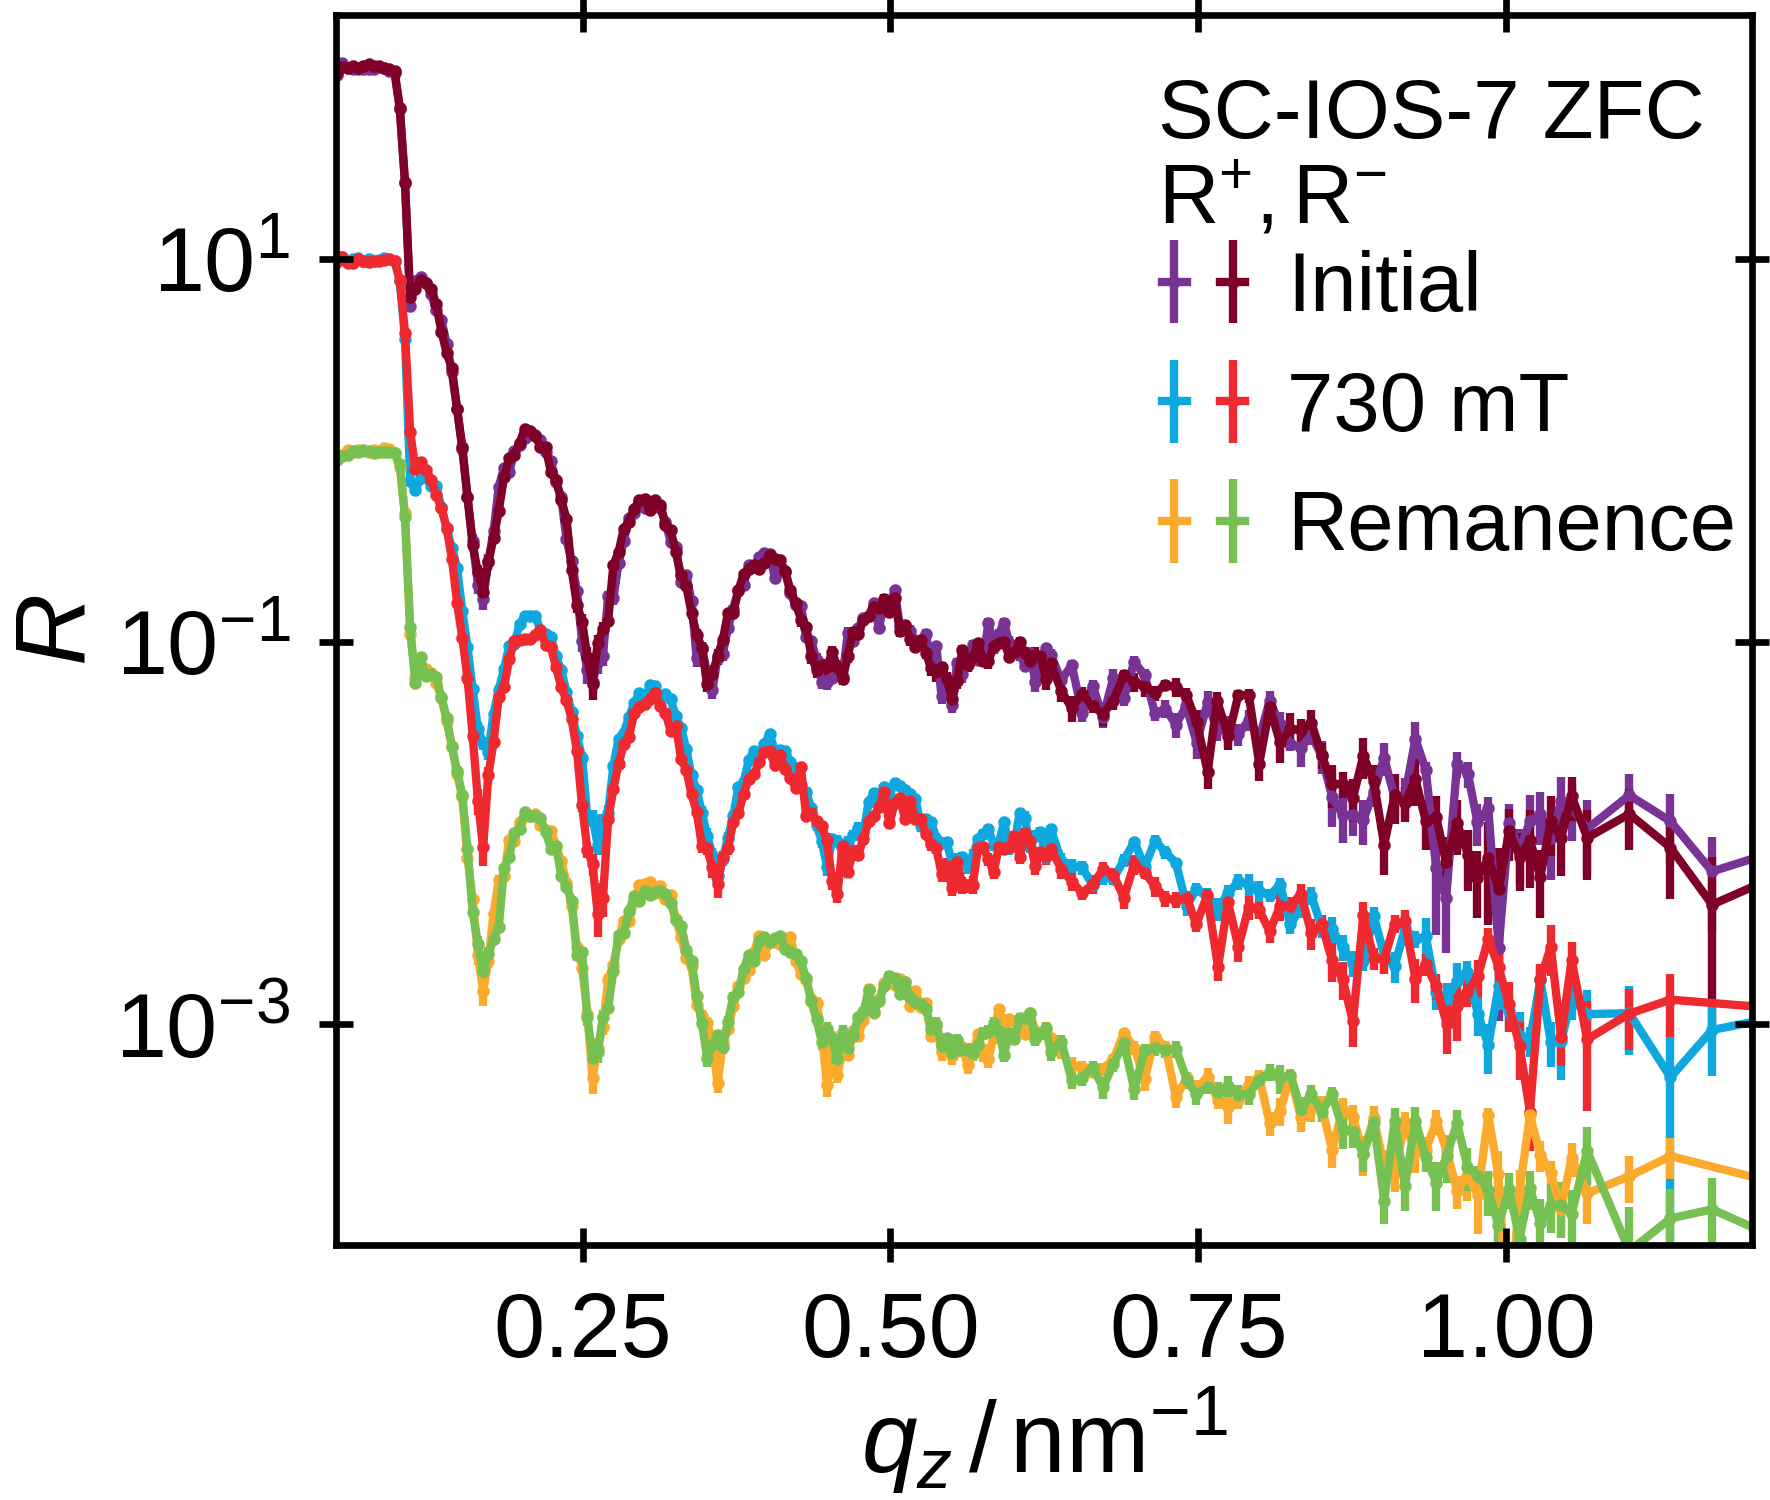
\includegraphics{looselyPackedNP_VerticalStructure_SC-IOS-7_PNR_ZFC30K}
    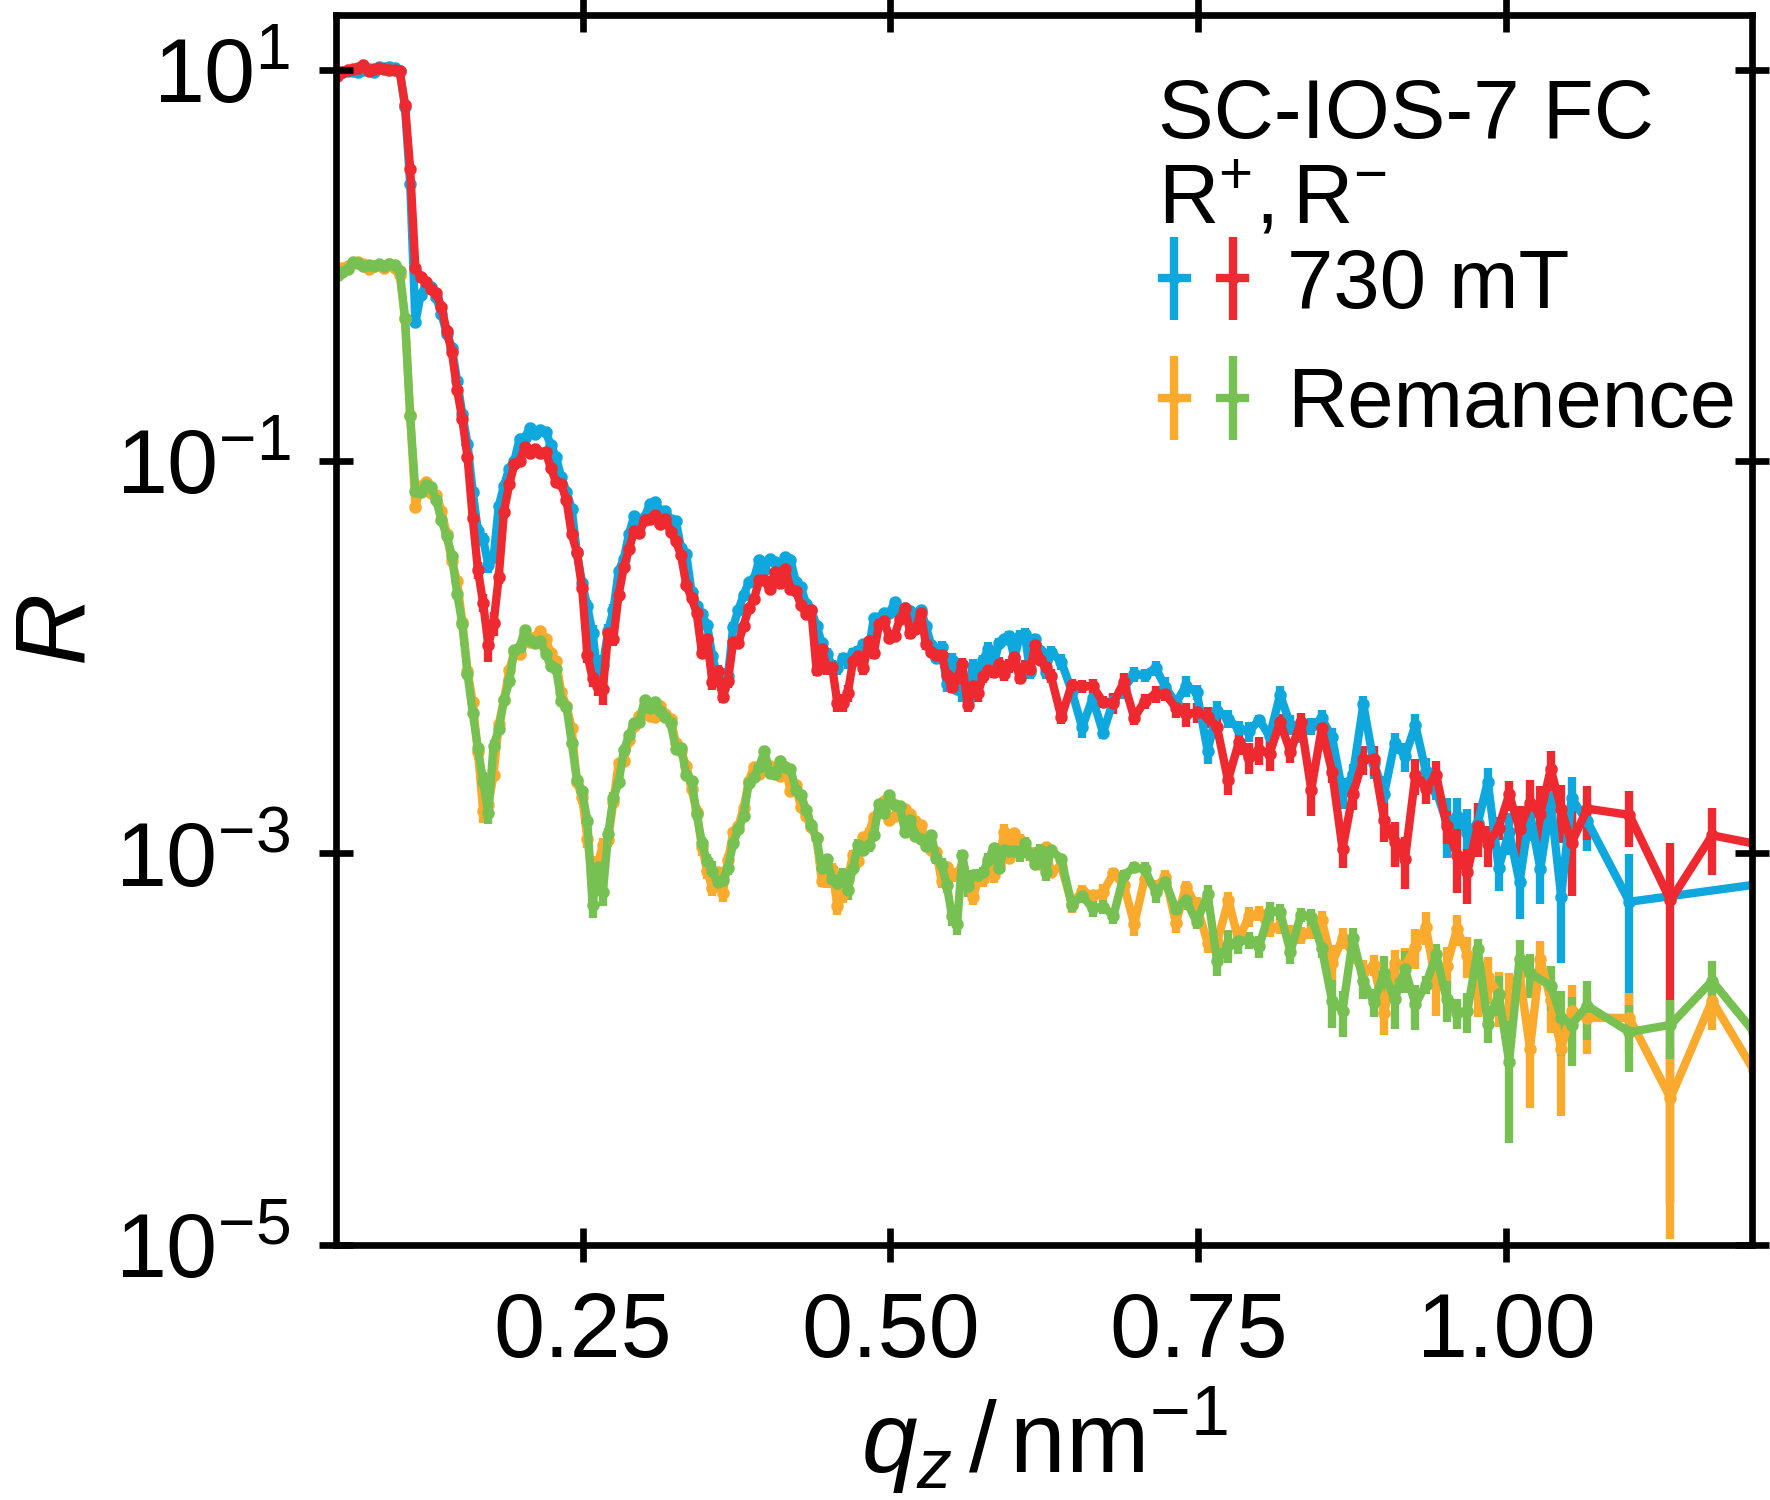
\includegraphics{looselyPackedNP_VerticalStructure_SC-IOS-7_PNR_FC30K}
    \caption{\label{fig:looselyPackedNP:layer:ZFCFCIOS7}Zero-field cooled (left) and field cooled reflectivity of SC-IOS-7 at a magnetic field of $730 \unit{mT}$ and in remanence. For the zero-field cooled the initial reflectivity after cooling at guide field is additionally shown.}
  \end{figure}

  For completeness, the zero-field and field-cooled reflectivities of SC-IOS-7 are shown in \reffig{fig:looselyPackedNP:layer:ZFCFCIOS7}.
  Similar to SC-IOS-11, the remanent reflectivity is in both cases similar to the state observed initially after zero-field cooling.
  The reflectivity measured at $730 \unit{mT}$ shows contrary to the room temperature measurement a very weak splitting between $R^{+}$ and $R^{-}$.
  However, the splitting is an order of magnitude smaller than what would be expected for a sample that is homogeneously magnetized with nanospheres in the order of $200 \unit{kA \, m^{-1}}$.
  This is contrary to the observation made with vibrating sample magnetometry in \refsec{sec:looselyPackedNS:layer:vsm} for SC-IOS-7.
  It was however not possible in the scope of this thesis to resolve why the nanospheres in SC-IOS-7 show no proper contrast in the reflectivity curves.
  Considering the bimodal nanosphere batch from which the samples were produced, no long-ranged order in the sample structure and the complex magnetism of magnetite from the oleate synthesis, there are too many complex variables to make a proper conclusion.
\end{document}